\documentclass{beamer}
\usetheme{metropolis} % Use metropolis theme

\renewcommand{\footnoterule}{%
  \hspace{10cm}
  \kern -3pt
  \hrule width \textwidth height 1pt
  \kern 2pt
}
\usepackage[utf8]{inputenc}
\usepackage[T1]{fontenc}
\usepackage[autostyle, english = british]{csquotes}
\usepackage[british]{babel}
\usepackage{todonotes}
\usepackage[%
  backend=biber,
  doi=false,
  url=false,
  isbn=false,
  eprint=false,
  style=authoryear,
  citestyle=verbose-note,
  hyperref=true,
  maxnames=99,
  minnames=1,
  maxbibnames=99,
  firstinits,
  uniquename=init]{biblatex}
%\DeclareFieldFormat[inproceedings, article]{pages}{}%
%\DeclareFieldFormat[inproceedings]{organization}{}%
\DeclareSourcemap{
  \maps[datatype=bibtex, overwrite]{
    \map{
      \step[fieldset=edition, null]
      \step[fieldset=publisher, null]
      \step[fieldset=pages, null]
      \step[fieldset=organization, null]
    }
  }
}

\addbibresource{../bibliography.bib}

\usepackage{caption}
\usepackage{xpatch}
\usepackage{bm}
\usepackage{amsmath}
\usepackage{mathtools} % for \mathclap
\usepackage{varioref}
\usepackage{siunitx}
\usepackage{hyperref}
\usepackage[noabbrev]{cleveref}
\newcommand{\creflastconjunction}{, and\nobreakspace} % use Oxford comma
\usepackage{todonotes}
\usepackage{phaistos}
\usepackage{multimedia}
\usepackage{tikz}
\usetikzlibrary{arrows, positioning, shapes.geometric}
\usetikzlibrary{calc}
\usepackage{pgfgantt}


\graphicspath{{../../figures/}}

\newcommand{\cn}{\footnote{\enquote{TODO: Citation.}, 2017, \textbf{Conference}, \textit{Author 1, Author 2, Author 3, Author 4} }}

\title{Deep-Learning-based Image Denoising in Ophthalmology\\GR kick-off}
\author{Lukas Krenz\\Advisor: Nicola Rieke\\Director: Prof.\ Dr.\ Nassir Navab}
\date{January 12, 2018} 
\institute{TUM, Chair for Computer Aided Medical Procedures \textit{\&} Augmented Reality}

\begin{document}
\maketitle

\begin{frame}
  \frametitle{Example Use-Case: Digital Window}
   \begin{figure}[h]
    \centering
    \missingfigure[figwidth=\textwidth]{Movie - Digital Window}
    \caption{Digital Window}
    \label{fig:digital-window}
  \end{figure}
\end{frame}


\begin{frame}{What are we trying to do?}
\begin{block}{Idea}
\begin{itemize}
\item Improve quality of retinal images
\item Should work in an intraoperative setting
\end{itemize}
\end{block}

\begin{block}{Use cases}
\begin{itemize}
\item Pre-processing for computer vision algorithms (e.g.\ vessel segmentation)
\item Provide improved quality for digital zoom.
\end{itemize}
\end{block}

\begin{block}{Constraints}
  \begin{itemize}
  \item Real-time
  \item Different levels of zoom
  \item Preserve structure of vessels etc.
  \end{itemize}
\end{block}
\end{frame}

\begin{frame}
  \frametitle{State of the Art}

\begin{block}{General Super-Resolution}
Many different super resolution approaches.
    
E.g. based on image statistics, self-simiarity of images, learned patch-databases or \textbf{convolutional neural networks}.

Only CNNs fulfil \textbf{both} quality and speed constraints
\end{block}


\begin{block}{Opthamology}
Use CNN-Upscaling\footcite{SaliencyGAN} 

Solid results, not optimized for intraoperative use-case
\end{block}
\end{frame}

\begin{frame}{Some common CNN-Topologies}
  \begin{figure}[h]
    \centering
    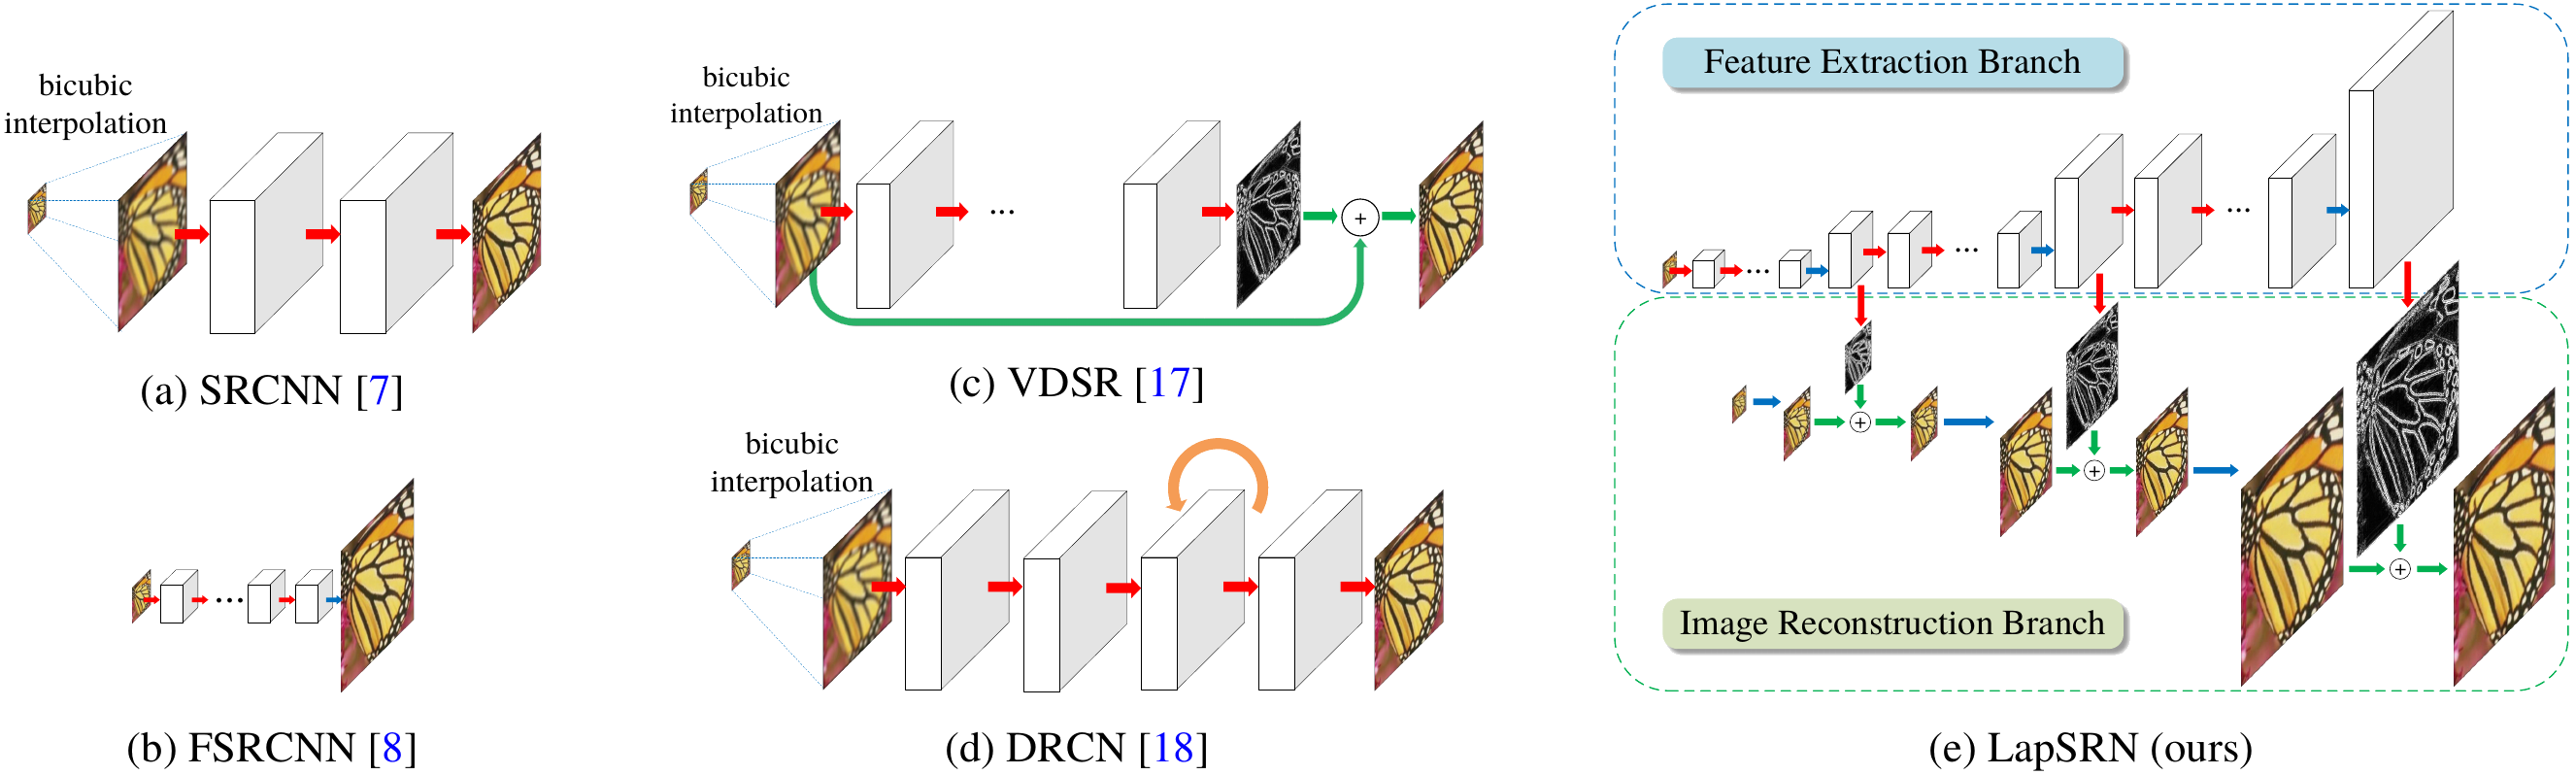
\includegraphics[width=\textwidth]{sr_architectures.png}
    \caption{Common Topologies\footcite{LapSRN}}
    \label{fig:lap-srn}
  \end{figure}
\end{frame}

\begin{frame}{Laplacian Network}
  \begin{figure}[h]
    \centering
    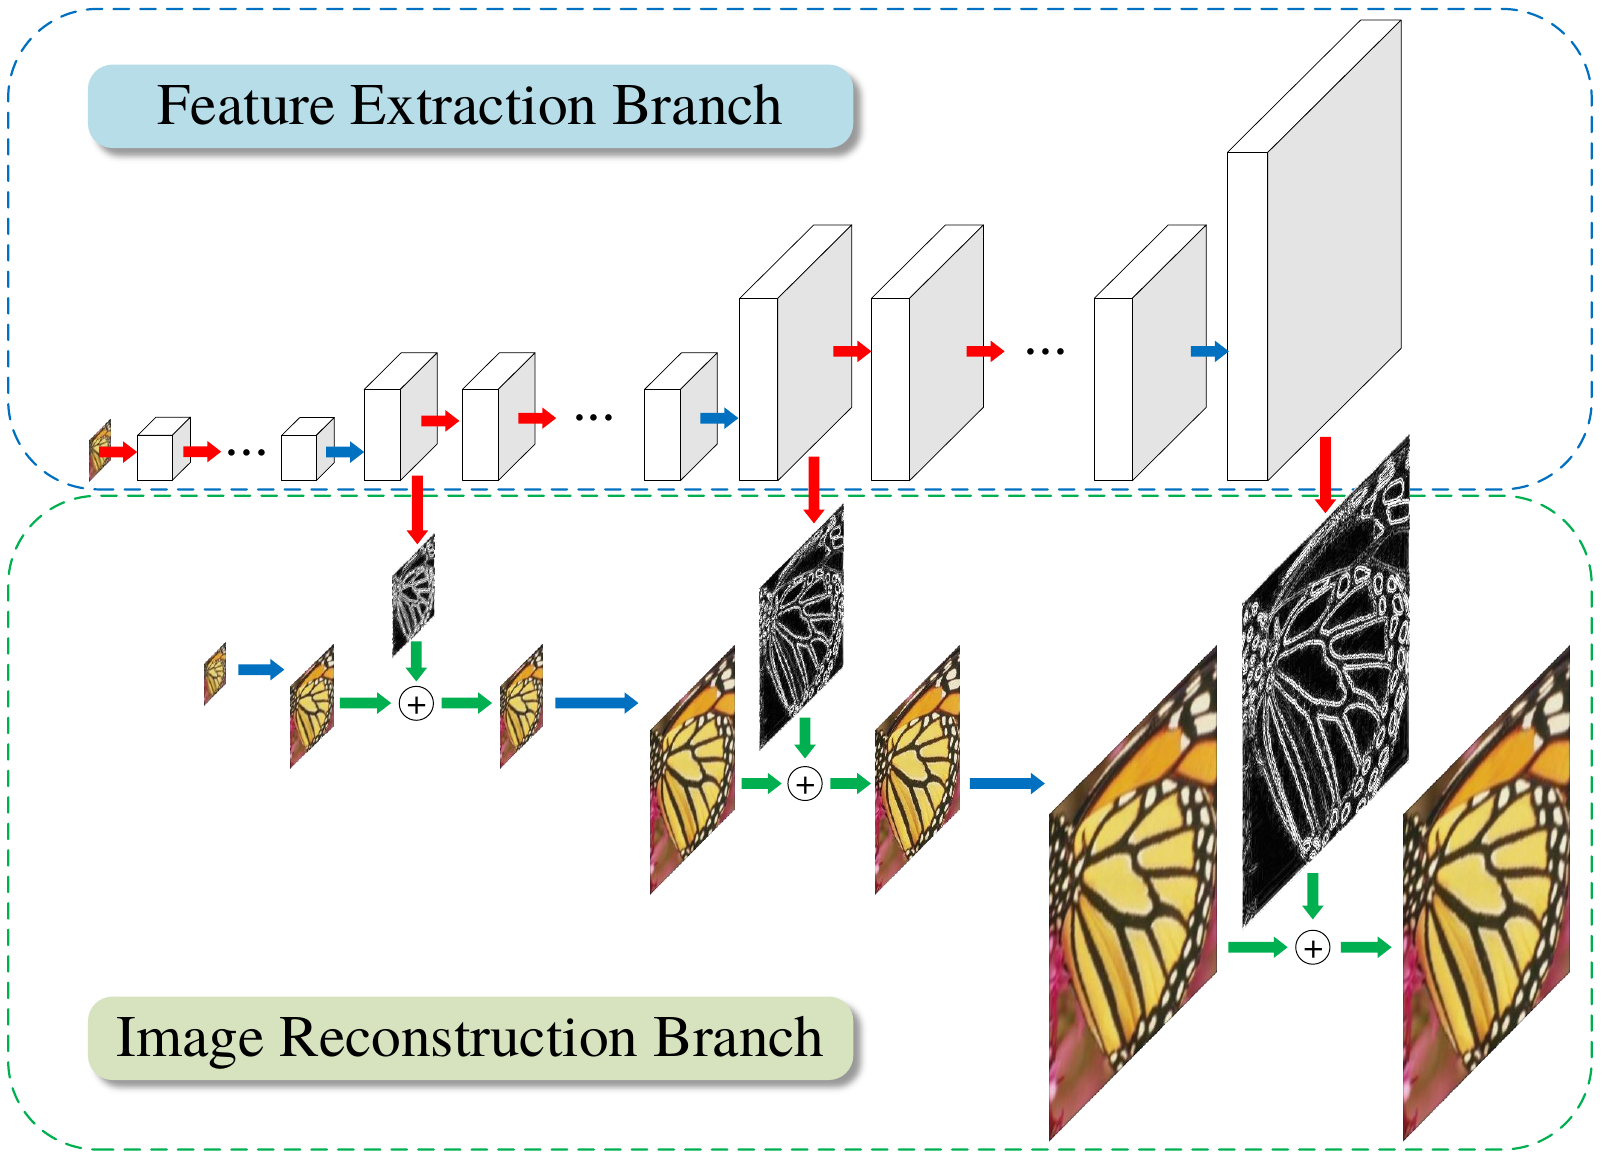
\includegraphics[width=0.7\textwidth]{lap_srn.png}
    \caption{Laplacian pyramid network\footcite{LapSRN}}
    \label{fig:lap-srn}
  \end{figure}
\end{frame}

\begin{frame}{Robust Loss}
(Relaxed) $L_1$  loss instead of $L_2$ loss
\begin{align*}
    \label{eq:charbonnier}
    L( \hat{\bm{y}}, \bm{y}; \bm{\theta}) &= \sum_n p \left( \bm{\hat{y}} - \bm{y} \right)\\
    %\shortintertext{with }
    p(\bm{x}) &= \sqrt{ \langle x, x \rangle  + \epsilon^2},
  \end{align*}

Robust, avoids \textbf{blurry} images\footcite{LapSRN}

\begin{columns}
  \begin{column}{0.33\linewidth}
    \begin{figure}[h]
      \centering
        
\includegraphics[width=0.9\textwidth]{loss_functions_lap_l2}
      \caption*{$L_2$ loss}
    \end{figure}
  \end{column}
  \begin{column}{0.33\linewidth}
    \begin{figure}[h]
      \centering
        
\includegraphics[width=0.9\textwidth]{loss_functions_lap_l1}
      \caption*{$L_1$ loss}
    \end{figure}
  \end{column}  \begin{column}{0.33\linewidth}
    \begin{figure}[h]
      \centering
        
\includegraphics[width=0.9\textwidth]{loss_functions_lap_gt}
      \caption*{Ground truth}
    \end{figure}
  \end{column}
\end{columns}
\end{frame}

\begin{frame}{Perceptual Loss---VGG-based}
Transform images before calculating loss, with feature map $\phi$:
\begin{equation*}
    L_p( \hat{\bm{y}}, \bm{y}; \bm{\theta}) = \Vert \phi( \bm{\hat{y}} ) - \phi( \bm{y}) \Vert
\end{equation*}

  \alert{Possibility 1}: Neural Network based loss, \textbf{automatic} features\footcite{PerceptualLoss}

  Extract feature maps from pre-trained VGG16-Network
\begin{columns}
  \begin{column}{0.33\linewidth}
    \begin{figure}[h]
      \centering
        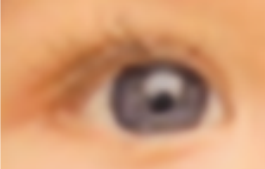
\includegraphics[width=0.9\textwidth]{perceptual_loss_l2}
      \caption*{$L_2$ loss}
    \end{figure}
  \end{column}
  \begin{column}{0.33\linewidth}
    \begin{figure}[h]
      \centering
        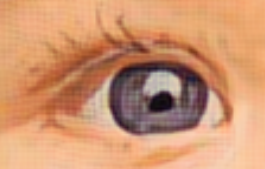
\includegraphics[width=0.9\textwidth]{perceptual_loss_vgg}
      \caption*{Perceptual loss}
    \end{figure}
  \end{column}  \begin{column}{0.33\linewidth}
    \begin{figure}[h]
      \centering
        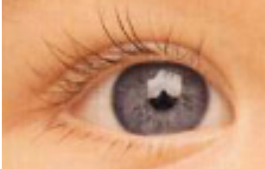
\includegraphics[width=0.9\textwidth]{perceptual_loss_gt}
      \caption*{Ground truth}
    \end{figure}
  \end{column}
\end{columns}
\end{frame}

\begin{frame}
  \frametitle{Perceptual Loss - Saliency Maps}
   Possibility 2: Saliency Maps\footcite{SaliencyGAN}

  \textbf{Handcrafted} features
\end{frame}

\begin{frame}{Adversarial Loss}
Two player game between generator (our network) and discriminator (which image is real?)\footfullcite{SRGAN}
\end{frame}

\begin{frame}{Possible Modifications for Network}
  Weight sharing (fewer parameters, robust filters, multi-scale training)

  Replace stacked convolutional layers with other layers (e.g.\ residual, recursive)

  Replace transposed convolutional layers with others (avoid checkerboard artifacts)\footfullcite{deconvolution}

  \begin{figure}[h]
    \centering
    %\includegraphics[]{}
    \caption{Example of block artifacts}
    \label{fig:lap-srn}
  \end{figure}
\end{frame}

\begin{frame}{Evaluation}
  Normally: Compare pixel-wise reconstruction error

  \textbf{Useless} in our case.

  Perceptual \textit{\&} adversarial loss improve perceived quality but increase MSE!

  Rather compare effectiveness as a pre-processing tool.
\end{frame}

\begin{frame} \frametitle{Timeline}
 \begin{figure}[ftbp]
  \centering
  \begin{ganttchart}[
    time slot format=isodate,
    x unit=0.40mm,
    today=2018-01-12,
    y unit chart=5mm,
    ]{2017-10-01}{2018-04-14}
\gantttitlecalendar{year, month} \\
\ganttbar{Pre-processing}{2017-10-19}{2018-02-01}\\
\ganttbar{Final Evaluation}{2018-02-15}{2018-04-15}\\
\ganttgroup{Coding}{2017-11-22}{2018-04-15}\\
\ganttbar{$L_1$-based Network}{2017-11-22}{2018-02-01}\\
\ganttbar{Perceptual Loss}{2018-01-22}{2018-03-15}\\
\ganttbar{Adversarial Loss}{2018-02-15}{2018-04-15}
\end{ganttchart}
\end{figure} 

\end{frame}
  
\begin{frame}{Summary}
\begin{itemize}
  \item Real-time super-resolution is realistic
  \item Selection of loss function is important
  \item Need for careful evaluation
\end{itemize}
\end{frame}

\end{document}